%; whizzy chapter
% -initex iniptex -latex platex -format platex -bibtex jbibtex -fmt fmt
% 以上 whizzytex を使用する場合の設定。

%     Tokyo Debian Meeting resources
%     Copyright (C) 2011 Junichi Uekawa
%     Copyright (C) 2011 Nobuhiro Iwamatsu

%     This program is free software; you can redistribute it and/or modify
%     it under the terms of the GNU General Public License as published by
%     the Free Software Foundation; either version 2 of the License, or
%     (at your option) any later version.

%     This program is distributed in the hope that it will be useful,
%     but WITHOUT ANY WARRANTY; without even the implied warranty of
%     MERCHANTABILITY or FITNESS FOR A PARTICULAR PURPOSE.  See the
%     GNU General Public License for more details.

%     You should have received a copy of the GNU General Public License
%     along with this program; if not, write to the Free Software
%     Foundation, Inc., 51 Franklin St, Fifth Floor, Boston, MA  02110-1301 USA

%  preview (shell-command (concat "evince " (replace-regexp-in-string "tex$" "pdf"(buffer-file-name)) "&"))
% 画像ファイルを処理するためにはebbを利用してboundingboxを作成。
%(shell-command "cd image201109; ebb *.png")

%%ここからヘッダ開始。

\documentclass[mingoth,a4paper]{jsarticle}
\usepackage{monthlyreport}
\usepackage{ulem}

% 日付を定義する、毎月変わります。
\newcommand{\debmtgyear}{2011}
\newcommand{\debmtgmonth}{10}
\newcommand{\debmtgdate}{22}
% (+ (* (- 2011 2005) 12) 9 -1) started from zero
\newcommand{\debmtgnumber}{81}

\begin{document}

\begin{titlepage}
\thispagestyle{empty}
% タイトルページ:編集必要な部分は最初のマクロに飛ばすこと

\vspace*{-2cm}
第\debmtgnumber{}回 東京エリア Debian 勉強会資料\\
\hspace*{-2cm}
\includegraphics[width=210mm]{image201003/debsen.eps}\\
\hfill{}\debmtgyear{}年\debmtgmonth{}月\debmtgdate{}日

% ここはアップデートすること
\rotatebox{10}{\fontsize{32}{32} {\gt 特集1: HaskellとDebianの辛くて甘い関係}}

\rotatebox{10}{\fontsize{32}{32} {\gt 特集2: 新連載!? 月刊 debhelper}}

\vspace*{-2cm}
\hfill{}
\includegraphics[height=6cm]{image200502/openlogo-nd.eps}
\end{titlepage}

\dancersection{Introduction}{上川 純一}

\begin{multicols}{2}
 

 今月のDebian勉強会へようこそ。これからDebianの世界にあしを踏み入れると
 いう方も、すでにどっぷりとつかっているという方も、月に一回Debianについ
 て語りませんか?

 Debian勉強会の目的は下記です。

 \begin{itemize}
 \item \underline{Debian Developer} (開発者)の育成。
 \item 日本語での「\underline{開発に関する情報}」を整理してまとめ、アップデートする。
 \item \underline{場}の提供。
 \begin{itemize}
  \item 普段ばらばらな場所にいる人々が face-to-face で出会える場を提供
	する。
  \item Debian のためになることを語る場を提供する。
  \item Debianについて語る場を提供する。
 \end{itemize}
 \end{itemize}		

 Debianの勉強会ということで究極的には参加者全員がDebian Packageをがりがり
 と作るスーパーハッカーになった姿を妄想しています。情報の共有・活用を通し
 て Debianの今後の能動的な展開への土台として、「場」としての空間を提供す
 るのが目的です。

\end{multicols}

\newpage

\begin{minipage}[b]{0.2\hsize}
 \definecolor{titleback}{gray}{0.9}
 \colorbox{titleback}{\rotatebox{90}{\fontsize{80}{80} {\gt デビアン勉強会} }}
\end{minipage}
\begin{minipage}[b]{0.8\hsize}
\hrule
\vspace{2mm}
\hrule
\begin{multicols}{2}
\tableofcontents
\end{multicols}
\vspace{2mm}
\hrule
\end{minipage}

\dancersection{事前課題}{前田 耕平}

今回の事前課題は以下です:
\begin{enumerate}
 \item 今、コンピュータを使ってあなたがやりたいこと、やっていることはなんですか?
 \item それはDebian(またはLinux)でできますか?Debian(またはLinux)を使ってなければその理由を教えて下さい。
\end{enumerate}
この課題に対して提出いただいた内容は以下です。
\begin{multicols}{2}
{\footnotesize
 \begin{prework}{ koedoyoshida }

\begin{enumerate}
\item $B;E;v$O$5$F$*$/$H$7$F!"<+Bp4D6-$G$O%5!<%P7O$O(BDebian$B!"%/%i%$%"%s%H7O$O(BWindows$B$K$7$F$$$^$9!#%5!<%P$K$O(BX$B$bF~$l$F$$$J$$$N$G(BGUI$B7OA`:n$O$9$Y$F(BWindows$B$H$$$&$3$H$K$J$j$^$9!#%/%i%$%"%s%H$G$d$C$F$$$k$3$H$,(BDebian$B$G=PMh$k$+$G$9$,(B...
  \begin{itemize}
  \item $B%a!<%k(B:Beckey:$B0JA0(B(Thunderbird 2.X)$B0\9T$r8!F$$7$?$1$l$I?6$jJ,$1%k!<%k(B($BF|K\8l(B($B$G$"$k(B/$B$G$J$$(B)$B$N%a!<%kH=JL!"J#9g>r7o$N(Band/or,from$B$*$h$S08@h(B(to/cc/bcc)$BH=JL(B)$B$,J#;($G(BTB$B$G:F8=$,$G$-$:0\9T:$Fq$GCGG0(B
  \item $B%V%i%&%6(B:$B%a%$%s%V%i%&%6$,(BOpera:$BB.EYLL$G(BFirefox(iceweasel)$B$h$j2wE,!#%5%V$O(BFirefox$B$H(BChrome$B$J$N$G(Biceweasel$B$H(BChromium$B$K0\9T$9$k$N$O$b$C$5$j$9$k$3$H0J30$OFC$KLdBj$J$7(B
  \item $B%(%G%#%?(B:$B=(4](B:Emacs$B$X0\9T$9$l$PLdBj$J$7(B
  \item $B%G%P%$%9%3%s%H%m!<%k(B:
    \begin{itemize}
    \item X Video Station:TV$BO?2h%5!<%P(B:$BBP1~%=%U%H%&%'%"$,(BWinowsXP$B$N$_!"%"%J%m%0J|Aw$,=*N;$7$?$N$G$*Lr8fLH$+$H;W$$$-$d!"(Bxvproxy(\footnote{\url{http://xvproxy.local.io/c5/}})$B$H%G%8%"%JJQ49$G<wL?$,1d$S$?!#(BGarapon TV$BEy$X0\9TM=Dj!#F0:n4F;k(B(EPG$B%A%'%C%/(B)$B$O(BDebian$B$K$F<B;\Cf(B
    \item Garapon TV:$B%o%s%;%0O?2h%5!<%P(B:Firefox$B$G1\Mw$7$F$$$k$N$G(Biceweasel$B$X0\9T2DG=!#F0:n4F;k(B($B%O%s%0%A%'%C%/Ey!"0[>o;~<+F0:F5/F0(B)$B$K$D$$$F$O(BDebian$B$K$F<B;\Cf(B
    \item Scansnap:$B<+?f(BPDF$B$r4IM}(B:$B0\9T2DG=$i$7$$$,>\:YL$D4::(B
    \item iPhone\&iPod:$B2;3Z$*$h$SF02h%i%$%V%i%j(B:$B0\9T2DG=$i$7$$$,>\:YL$D4::(B
    \end{itemize}
  \end{itemize}
\end{enumerate}
\end{prework}

\begin{prework}{ sheeta38 }

\begin{enumerate}
\item $B<x6H!J%W%m%0%i%_%s%0F~Lg#1!K$N%l%]!<%H:n@.!#!!(Bgcc$B$H(B \LaTeX $B$rMQ$$$F$$$k(B
\item $B%W%m%0%i%_%s%0!"$*$h$S(BLinux$B$K$b$C$H?($l$k!#8=>u!"%3%s%T%e!<%?$K4X$7$FCN$C$F$$$k$3$H$,$"$^$j$K>/$J$$$H46$8$F$*$j!"$3$l$i$K?($l$F$$$/$3$H$G!">/$7$:$D8*$r$J$i$7$F$$$-$?$$!#(B

C$B8@8l$b(B\LaTeX$B!"$"$k$$$OB>$N8@8l(B(Ruby, Python$BEy(B)$B$b!"(BWindows$B$G4D6-$r@0$($h$&$H$9$l$P2DG=$@!#$?$@$7(BLinux$B$NJ}$,4D6-9=C[$,MF0W$G$"$k$H;W$&!#(B
$BB>$K6qBNE*$J(BLinux(Debian)$B$NMxE@$,$"$k$J$i$PCN$j$?$$!#(B
\end{enumerate}

\end{prework}

\begin{prework}{ r.matsumiya@syntaxerror.biz }

$B3+H/%a%$%s!"%l%]!<%H:n@.!#N>J}$H$b(BDebian$B;H$C$F$^$9!#(B
\end{prework}

\begin{prework}{ $B5HLn(B(yy\_y\_ja\_jp) }

$BK?<R@=%*%U%#%9%9%$!<%H$N%U%!%$%k$r%l%$%"%&%H$r2u$5$:I=<(!&JT=8$7$?$$$G$9!#(B

\end{prework}

\begin{prework}{ $B%-%?%O%i(B }

$B;~4V%.%j%.%j$J$N$G!">-Mh$d$j$?$$$3$H$G!"(BLinux$B$@$H(B
$B$d$j$K$/$=$&$J$b$N$r$"$2$F$_$k!#!J$h$$J}K!$,$"$l$P65$($F$/$@$5$$!#!K(B
\begin{enumerate}
\item $BCO%G%8$NO?2h(B \\
$B?'!9J}K!$,$"$k$h$&$G$9$,!"%3%s%F%s%DJ]8n$H$+$GLLE]$=$&(B
\item $B<+?f%3%s%F%s%D$N:n@.(B\\
$B%9%-%c%s$O$G$-$=$&$@$,!"(BOCR$B$H$+%9%-%c%JIUB0$N$*$^$1$KIi$1$F!"(BWindows$B$r;H$$$=$&$J5$$,!D!D!#(B
\end{enumerate}

\end{prework}

\begin{prework}{ $BLZB<(B $BM[0l(B }

Debian$B$G(BApache+SQLite+PHP$B$J(BWeb$B%"%W%j3+H/$r$7$F$$$^$9!#$=$m$=$m(BC\#$B$d(BVB.NET$B$b$d$j$?$$$H;W$C$F$$$^$9$,!"(BMono$B$N(BVB.NET$B%3%s%Q%$%i$OIT0BDj$G5!G=$,==J,$G$J$$$N$G(BWindows$B4D6-$r(BVM$B$KMQ0U$7$F3+H/$7$h$&$H;W$C$F$$$^$9!#(B
\end{prework}

\begin{prework}{ dictoss($B?yK\!!E5=<(B) }

\begin{itemize}
\item web$B1\Mw!"%a!<%k!"%W%m%0%i%`3+H/$O;E;v$b<+Bp$b(BDebian GNU/Linux$B$G9T$C$F$$$k(B
\item MIDI$B%-!<%\!<%IN}=,$O(BWindows$B$r$R$H$^$:;H$C$F$$$k!#(B(Linux$B$G$b$G$-$k$H;W$&$,$"$^$jD4$Y$F$$$J$$$?$a(B)
\item $B%S%G%*O?2h(B(PT2$B$r;HMQ(B)$B$O(BFreeBSD$B$G9T$C$F$$$k!#<+Bp(Bweb$B%5!<%P$,(BFreeBSD$B$@$C$?$N$G!"$=$l$KAj>h$j$9$k7A$G$=$N$^$^;H$$B3$1$F$$$k$+$i(B
\end{itemize}

\end{prework}

\begin{prework}{ Kiwamu Okabe }

Haskell!Debian$B$,:G$bE,$7$F$$$^$9(B!

\end{prework}

\begin{prework}{ $BED86M*@>(B }

$B%3%s%T%e!<%?$r;H$C$F$d$j$?$$$3$H$G$"$j!"$d$C$F$$$k$3$H$O;E;v$H$+%$%s%?!<%M%C%H$r;H$C$?$j$H$+!#(BDebian$B$r;H$C$F$G$-$F$$$^$9!#(B

\end{prework}

\begin{prework}{ Arnaud Fontaine }

I'm a Debian developer who arrived in Tokyo last year and interested in meeting up some other developers. I'm using Debian only at work and home.

\end{prework}

\begin{prework}{ Hirotaka Kawata }

\begin{enumerate}
\item $B<qL#$G(B Python $B$G4JC1$J%W%m%0%i%`$N:n@.$d!"%"%;%s%V%i(B(binutils)$B$d%3%s%Q%$%i(B(gcc)$B$N?7$7$$%"!<%-%F%/%A%c$X$N0\?"!#;E;v$G(B PHP, Rails $B$d(B HTML, CSS $B$r$D$+$C$?(B Web $B%W%m%0%i%`$N:n@.!#M7$S$G%2!<%`$H$+(B($B%U%i%$%H%7%_%e%l!<%?$J$I(B)
\item $B$G$-$k(B
\end{enumerate}

\end{prework}

\begin{prework}{ mitty }

$B%U%!%$%kEy$N%P%C%/%"%C%W$d=EJ#4IM}$r$b$C$H3Z$K$7$?$$!#(B

$BIaCJ;H$$$N(BPC$B$H$OJL$K!"%U%!%$%k%5!<%P(B(NAS)$B$H$7$F(BUbuntu$B$rMQ$$$F$$$k$,!"%P%C%/%"%C%W$d@$Be2=!"%@%&%s%m!<%I$7$F$-$?(Biso$B%$%a!<%8$J$I$N%U%!%$%k=EJ#%A%'%C%/$J$I!"$[$H$s$IE,59<jF0$G$d$C$F$$$k$?$a!"$"$kDxEY<+F02==PMh$k$H4r$7$$!#(B
\end{prework}

\begin{prework}{ osamu@debian.org }

Debian$BJ8=q$N@0M}!J(BDDP$B$N(BXETEX$BBP1~(B)$B!"FbMF99?7!!!<!!;HMQM}M3!'!!<+L@(B

$B<B:]$O;dJ*$N<L??$NJT=8!&@0M}$0$i$$$,(BDEBIAN$B!VMxMQL\E*!W$G$9!#!!!<!!B>$N%W%i%C%H%U%)!<%`$O$9$0>C$($F$$$/$,!"$$$D$b:G?7%7%9%F%`$G$$$i$l$k$7%3%s%s%Q%F%#%S%j%F%#!<$N?4G[$,$J$$!#$J$s$H8@$C$F$b$*6b$,$+$+$i$J$$!#$3$s$J=j$,M}M3$G$9!#(B

$B@5D>$J$H$3$m!"%V%i%&%6!<$r;H$&0J30$O0U30$H(BDEBIAN$B$r;H$C$F$$$^$;$s!#(BDebian$B$O>/!99S:o$j$G$9$,!";H$$$d$9$$$N$H!":#$^$G$N=,47$G;H$C$F$$$^$9!#:G=i$OF|K\8l%5%]!<%H$G$-$k$,%Y!<%9$,1Q8l$H$$$&$N$,M}M3$G$7$?$,!"$$$^$H$J$C$F$O(BUBUNTU$B$r$J$<;H$o$J$$$+$H$J$j$^$9!#$^$"!"$"$($F$$$($P<+J,$?$A$G:n$C$F$$$k$H$$$&5$$,$9$k$N$,M}M3$G$9$+$M!#(B
\end{prework}

\begin{prework}{ pi8027 }

\begin{enumerate}
\item \begin{itemize}
\item $B%W%m%0%i%`!">ZL@!"J8=q$J$I$N:n@.(B
\item $B9V5A$N%N!<%H$r<h$k:n6H!"%l%]!<%H$r:n@.$9$k:n6H(B
\item $B>pJs<}=8(B
\item $B<+J,<+?H$K4X$o$k?'!9$JJ*;v$N4IM}(B($BM=Dj4IM}$H$+(B)
\item $B$3$l$i$N:n6H$NItJ,E*$b$7$/$O40A4$J<+F02=(B
\end{itemize}
\item $B$G$-$^$9(B
\end{enumerate}

\end{prework}

\begin{prework}{ taitioooo$B!JD9C+@n!K(B }

$B2H$N(BKVM$B$d(BXenserver$B$r4IM}$G$-$k%;%k%U%]!<%?%k@0Hw$7$h$&$H$7$F$$$^$9!#(BLinux$B$G$G$-$^$9$,!"(Bdebian$B$G$G$-$^$;$s!#(BCentos$B;H$C$F$^$9!#(B

\end{prework}

\begin{prework}{ $BLnEg!!5.1Q(B }

\begin{enumerate}
\item \begin{enumerate}
\item $B<+J,FH<+;EMM$N%/!<%k$J(BGUI$B$H%/!<%k$JF~=PNO%G%P%$%9$r;}$D%/!<%k$J(BPC/$B%b%P%$%k5!$r:n$C$F?M$K<+K}$9$k(B
\item $B$H$K$b$+$/$K$b%/!<%k$JGz0B(BPC/$B%b%P%$%k5!$r:n$C$F<R2qE*!?7P:QE*$K87$7$$$H$3$m$G$H$K$+$/N.9T$i$;$k!#%3%s%F%s%D:n$i$;$k!#$*6b$^$o$9(B
\end{enumerate}
\item $B$$$d!"$=$N!#(BDebian(Linux)$B0J30$@$H$+$J$jFq0WEY9b$$$C$9$h$M!)(B\\
$B"(CfG/$K$J$C$F$+$i!"?_FsIB45$C$F$^$9(B...
\end{enumerate}
\end{prework}

\begin{prework}{ $B$^$($@$3$&$X$$(B }

  \begin{enumerate}
  \item $B$d$j$?$$$3$H$O!"<+J,$d2HB2$N@83h$rJXMx$K$9$k$3$H(B
  \item $B$3$^$a4F;k%+%a%i$J$I!"ItJ,E*$K$O=PMh$F$$$k$1$I!"$^$@40A4$G$O$J$$!#:#$N6PL3@h$b(BCentOS$B$d(BUbuntu$B$G!"(BDebian$B$O;H$C$F$J$$!#A0<T$O5;=QE*(B($B%O!<%I%&%'%"(B)$B$d%j%=!<%9(B($BMW$O<+J,$N;~4V$H6b(B)$B$NLdBj!"8e<T$O@/<#E*!"?ME*$JM}M3(B
  \end{enumerate}
  Debian$B$@$1$J@83h$rAw$k$?$a$K!"4hD%$k$N$G$9!#(B
\end{prework}



}
\end{multicols}

\dancersection{最近のDebian関連のミーティング報告}{前田 耕平}
\subsection{東京エリアDebian勉強会80回目報告}

9月の東京エリアDebian勉強会は、最初の3連休の1、2日目の土日に伊東の山喜旅館さんで温泉合宿、通称Debian温泉2011を開催しました。参加者は8名。今年は15時にチェックインしてから、翌朝の4-5時まで黙々とやるガンバルマン大会になりました。吉田さんが差し入れしてくれた日本酒もあったのに、誰一人酒を飲まず、温泉も早朝寝る前か、7時前の起床直後に入る、というストイックさ。温泉行っているのにもったいないですね。

各人それぞれの作業を行った以外、Mini DebConfについてのディスカッションも行いました。Mini DebConfについては今後の進め方の方針も決まったので、良い成果を出せたと言えるでしょう。F2Fでその場で聞けて、集中して作業&討議できる環境というのは重要ですね。

翌日は、温泉入って朝食後、伊東駅で解散しました。次回はどこでしょうか。お楽しみに。

% (query-replace-regexp "<.*?>" "")
% (query-replace-regexp "^[	 ]\+" "")



\dancersection{Debian Trivia Quiz}{前田 耕平}

ところで、みなさん Debian 関連の話題においついていますか?Debian関連の話
題はメーリングリストをよんでいると追跡できます。ただよんでいるだけではは
りあいがないので、理解度のテストをします。特に一人だけでは意味がわからな
いところもあるかも知れません。みんなで一緒に読んでみましょう。

今回の出題範囲は\url{debian-devel-announce@lists.debian.org} や \url{debian-devel@lists.debian.org}に投稿された
内容とDebian Project Newsなどからです。

\begin{multicols}{2}
 %; whizzy-master ../debianmeetingresume201101.tex
% 以上の設定をしているため、このファイルで M-x whizzytex すると、whizzytexが利用できます。
%
% ちなみに、クイズは別ブランチで作成し、のちにマージします。逆にマージし
% ないようにしましょう。
% (shell-command "git checkout quiz-prepare")

\santaku
{Debian温泉2011の1日目はいつでしょうか?}
{9/17}
{9/18}
{9/19}
{A}
{さっきの話を聞いていればわかって当然ですね}

\santaku
{8月にDebianは誕生日を迎えました。何周年でしたでしょうか?}
{17}
{18}
{19}
{B}
{今年もお祝いしましたよね}

\santaku
{最新のDebian Newsはいつ発行されたでしょうか?}
{9/17}
{9/18}
{9/19}
{C}
{購読していれば知っていて当然ですね}

\santaku
{10/17の''delegation for the DSA team''で代表団に任命されなかったのは誰でしょう?}
{Faidon Liambotis}
{Luca Filipozzi}
{Nobuhiro Iwamatsu}
{C}
{他に任命されたのは、の全部で合計名です。}

\santaku
{Wheezyフリーズの予定はいつでしょう?}
{2012年4月}
{2012年6月}
{2012年8月}
{B}
{あと6ヶ月ですよ!}

\santaku
{1.16.1がリリースされたdpkgに該当するのはどれ?}
{\texttt{dpkg-buildpackage}コマンドでは \texttt{CFLAGS, CXXFLAGS, LDFLAGS, CPPFLAGS, FFLAGS}の\texttt{export}が必須になった}
{\texttt{dpkg-deb}コマンドに\texttt{--verbose}オプションが追加された}
{Multi-Archフィールドがサポートされた}
{B}
{\texttt{dpkg-buildpackage}ではこれらのオプションが不要になりました。Multi-Archは1.16.2からサポートされる予定です。\texttt{dpkg-deb -x/--extract -v/--verbose}で\texttt{dpkg-deb -X/--xextract}と同じ動きをするようになりました。}

\end{multicols}



%-------------------------------------------------------------------------------
\dancersection{Debian とはなにか?}{岩松信洋}
%-------------------------------------------------------------------------------
\index{debian}

今回はDebian勉強会を筑波大学さんで行うということで、たぶんLinuxやUbuntu、
Fedoraという言葉は知っているけど、
Debianは知らないって方がいると思います。
簡単にDebianとは何なのかを簡単に説明します。

\subsection{Debianとは?}

Debian Project の略称、またはDebian OSそのものを指す場合があります。
フリーかつオープンなOSを作る完全ボランティアベースのプロジェクトです。
歴史が長く保守的なLinuxディストリビューションの一つです。

公式開発者は約1000名。非公式な開発者やパッケージメンテナ、翻訳者などを入れると
5000名以上になります。世界のいたるところに開発者がいて、日本では約30名ほど公式
開発者が活動しています。また、日本の開発者が集まって活動している Debian JP Project
もあり、日本でのDebian環境のサポート、開発者育成、ユーザサポートなどを行なっています。

オープンソース・ライセンスの要件の定義(The Open Source Definition(OSD))は
DebianのDebianフリーソフトウェアガイドラインをベースとしたものです。

\subsection{特徴}

\subsubsection{フリーなソフトウェアで構成されている}
Debian プロジェクトはフリーソフトウェアを強く支持しています。
ソフトウェアには、いくつもの違ったライセンスが使われるので、 
Debian フリーソフトウェアガイドライン (DFSG) を作って、 
何をもってフリーソフトウェアと言えるのかの妥当な定義をしています。 

\begin{itemize}
\item 何台のマシンにもソフトウェアをインストールしても良い。
\item 何人の人がソフトウェアを同時に使用しても良い。
\item 何個でもソフトウェアのコピーを作ってもいいし、それを誰にあげても構わない。(フリーもしくはオープンな再配布)
\item ソフトウェアの改変に対する制約が無い。(特定の通告を変えない事を除く)
\item そのソフトウェアを配布や売る事に対する制約が無い。
\end{itemize}

Debian の「main」ディストリビューションには、DFSG に適合したソフト
ウェアしか 入れる事を許されていません。
\footnote{http://www.debian.org/intro/free.ja.html より}

とはいっても、フリーではないアプリケーション
を使いたいユーザもいるので、そのようなユーザのためにcontrib、non-free 
といったパッケージセクションを作って、できるだけ提供できるようにしています。

\subsubsection{オープンな開発をしている}
完全ボランティアの団体なので、特定の企業の力によってDebianの
方針が変更されたりすることがありません。
バグや議論経過なども全て公開されており、プロジェクトの方針等
はDebian公式開発者の選挙によって決まります。

\subsubsection{バイナリベースのディストリビューション}
ディストリビューションにはバイナリベースとソースベースの2種類があります。
前者は既にコンパイルされたパッケージを提供するディストリビューションで、
Debian や Redhat、Ubuntuなどがあります。
既にコンパイルされているので、直ぐに使うことができますが、一定のルールに
よって最適化されているため、
使っているCPU向けに最適化されているとは限りません。しかし、同じアーキテク
チャならどの環境でも同じ問題が再現する
可能性があり、問題の共有が容易になります。
自分で使うソフトウェアは自分でコンパイルするというディストリビューションで、
代表的なものとしてGentooがあります。
パケージにはソースコードはなく、コンパイルに必要な簡単なスクリプトがパッケー
ジに同梱されています。
このスクリプトで定義されている場所からソースコードをダウンロードし、コンパイルします。
これは自分に合わせたソフトウェアに最適化できるという利点があります。そのかわり
ソフトウェアを使うには時間がかかり、
問題があった場合でも他の環境では再現しにくいというデメリットもあります。

\subsubsection{豊富なパッケージ数}

Debianは多くのパッケージを提供しており、現在約3万パッケージのパッケージが利用可能です。
他のディストリビューションは、Gentooが15000パッケージ、Ubuntuだと10000パッケージ
\footnote{main と Universe がありますが、基本的にUbuntu側のサポートありなのはmainのみ。} 
ほどあります。
Debian の変態的なところは、各アーキテクチャで同じバージョンのバイナリを
提供している事です。
リリース対象になっているアーキテクチャでパッケージが動作しない場合、ポーティング
を行い、開発元に取り込むように提案します。

%Gentoo? 約15000。あんなのビルドできるかわからないものも多くあるのでだめだろ。
%Ubuntu? main だけだと5000ぐらい?Universe とかありますが、基本的にUbuntu側のサポートはなし。

\subsubsection{ポリシーに基づいたパッケージ}
Debian で提供されているパッケージは Debian Pocilyという
パッケージングポリシーに基づいて作成されています。
このポリシーは厳格に決められており、違反しているパッケージ
はDebianにインストールされません。

\subsubsection{強力なパッケージングシステム}
Debianでは パッケージングシステムに dpkg というアプリケーションを使っており、deb という拡張子
がついたパッケージファイルをインストール、アンインストールします。
パッケージの依存関係管理がしっかりされており、depends(依存)、recommends(推奨)、
suggests(提案) などの項目によってコントロールしています。
パッケージマネージャのAPT (Advanced Package Tool) によって、インストールしたいパッケージに
依存しているパッケージがインストールされます。アンインストールも同様です。

\subsubsection{アップデートが容易}
Debian は約2年毎に安定版がリリースされます。Debian は 
前回のバージョンからのアップデートをサポートしています。
例えば、2007年にリリースされた 4.0 から、最新版の 6.0 にアップデートするには、
4.0、5.0、6.0 と順にアップデートすることによって可能です。

\subsubsection{豊富なサポートCPUアーキテクチャ}
現時点で正式サポートCPUアーキテクチャは11、次期リリースに向けてサポート
準備中が 10 あります。
サーバからPC、組み込みCPUまでサポートしています。
新しいCPUアーキテクチャをサポートするためのインフラもあるので、何がサポートしたいCPUが
ある人、debian-ports プロジェクトに連絡するとインフラを提供してくれるかもしれません。


\begin{minipage}[t]{0.5\hsize}

現在サポートしているアーキテクチャ。
\begin{itemize}
  \item amd64
  \item armel
  \item hurd-i386
  \item i386
  \item ia64
  \item kfreebsd-amd64
  \item kfreebsd-i386
  \item mips
  \item mipsel
  \item powerpc
  \item s390
  \item sparc
\end{itemize}

\end{minipage}
\begin{minipage}[t]{0.5\hsize}

サポート予定のアーキテクチャ
\begin{itemize}
  \item alpha
  \item armhf
  \item avr32
  \item hppa
  \item m68k
  \item powerpcspe
  \item s390x
  \item sh4
  \item sparc64
\end{itemize}

\end{minipage}

\subsubsection{Linux以外のカーネルもサポートする}

LinuxをカーネルとしたOS、Debian GNU/Linux だけではなく、
FreeBSDのカーネルを使ったOS Debian GNU/kFreeBSD 
も提供しています。
Debian 開発者の中にはGNU Hurd, Minix, NetBSD カーネルを
ベースにした Debian を開発している人もいます。

\subsubsection{他のOSSプロジェクトと関連が強い}

Debian開発者と各OSS開発者が兼務していることが多く、他のOSS
プロジェクトと結び付きが強いです。パッケージメンテナ=開発元の開発者
ということが多いのが特徴です。自分の作ったソフトウェアをDebianに入れたい人が
多いようです。
また、大抵のDebian開発者は複数のプロジェクトに顔を出しているので、更にプロ
ジェクト間の結びつきが強いです。

\subsubsection{派生しているディストリビューションの多さ}
いままで説明した特徴によって、Debianから派生したディストリビューションが多く
あります。
有名なところでは、UbuntuやKnoppix、Vyatta (VPN/ネットワークファイアウォール)
などがあります。
現時点で129以上の派生ディストリビューション
\footnote{http://distrowatch.com/dwres.php?resource=independence 参照}
があり、Debianの live CD システムを使った小さい
ディストリビューションを入れるともっと多くなります。
また派生として分散させているだけでなく、派生したディストリビューションの
成果を本家であるDebianに取り組む仕組みもあります。
ちなみに2番目に多いのはFedoraベースの 63 です。

\subsection{まとめ}

\begin{itemize}
\item フリーである。
\item オープンな開発プロジェクトである。
\item 世界規模のボランティアベースのプロジェクトである。
\item バイナリベースのディストリビューションで、サポートしているパッケージ数が多い。
\item サポートしているアーキテクチャが多い。
\item Linux カーネルだけをサポートしていない。
\item 派生しているディストリビューションが多い。
\end{itemize}

\subsection{んで、どういう風に使えばいいの?}

個人的な見解ですと、

\begin{itemize}
\item 開発に使いたいなら、Debian か Gentoo。

アップストリームに近い位置にいるためです。
パッチなどがディストリビューション開発者経由で取り込まれやすい。

\item デスクトップやノートPCで使いたいなら Ubuntu。いろいろデスクトップとか弄りたいなら、DebianかGentoo。

2ch とかニコニコ動画みる程度なら Ubuntu で十分だと思います。もちろん Debian でも問題ありません。
プログラムを最適化したいとか、「Gnomeとかイラネ!他のデスクトップ環境が欲しい」という人なら、Debian かGentooをお薦めします。

\item サーバで使いたいなら、Debian。

無駄なものがインストールされてないから。

\end{itemize}
です。

ぜひDebianを使って、フィードバックをください。
そして開発に興味がある人は開発に参加してみてください。手取り足取り教えます。
みんなでDebianを良いものにしていきましょう。


%-------------------------------------------------------------------------------
\dancersection{HaskellとDebianの辛くて甘い関係}{岡部究}
%-------------------------------------------------------------------------------
\index{haskell}

\subsection{Haskellというプログラミング言語}

Haskell \footnote{\url{http://haskell.org/}}
というプログラミング言語をご存知でしょうか。
Haskellは関数型言語の一種で以下のような特徴があります。(以下の意見はHaskell初心者である筆者の偏見や間違いを多量に含んでいます)

\begin{itemize}
\item 静的型付け

暗黙の型変換とかそんなことは起きません。
また多くのエラーをコンパイル時に検出することができます。
Haskellでプログラミングをしていると視野角が狭くなる気分になると思います。
型で守られることによって「考慮に入れておくべき前提」のコード範囲が小さくなり、
そしてインターフェイスに用いている型について「本当にこれがふさわしいのか?」
と考えることになります。
もっと簡単に言うと「型による設計」をHaskellでは行います。

\item 型推論

型をすべて書く必要がないという利点もありますが、
型推論がないと綺麗に表現できないこともあります。
個人的には、関数自体には型を書いて、関数の内部での型は省略することが行儀が
良いと思います。

\item パターンマッチ

\texttt{if}や\texttt{case}文で場合分けを記述するよりもはるかに柔軟な場合分けができます。
アルゴリズムの記述とはある種場合分けの繰り返しとも言えるので、
この場合分けを型で記述できると、わかりやすく簡潔になります。

\item 遅延評価

諸刃の剣ですが、無限リストを作れたり、破壊的なデータ構造を用いなくても計算量を
少なくすることができます。
正格性フラグを使うことで遅延評価を部分ごとに抑制することもできます。

\item コンパイルして実行

ローカルでコンパイルすれば、配布先にはHaskellがインストールされていなくても
OKです。要は単なる実行バイナリになります。
また\texttt{runhaskell}コマンドでコンパイルせずに実行することもできます。

\item 読みやすく、書きやすい文法

本当です!
もし型を使っても不足なケースではTemplate Haskell
\footnote{\url{http://www.kotha.net/ghcguide_ja/latest/template-haskell.html}}
を使えばコンパイル時にメタプログラミングをすることもできます。
個人的には見た目があまりにかわりすぎてしまうので、邪悪なのではないかと
思っていますが。。。まぁ使いどころに気をつけましょう。

\end{itemize}

どうでしょう。わくわくしますよね!
さっそく使ってみましょう。なぁにDebianなら簡単です。\footnote{ここではDebian Sidを使っていることを前提にしています。}
haskell-platformパッケージをインストールすればHaskellコンパイラであるghcと
その基本ライブラリ群が使えるようになります。
Rubyのirbコマンドや、Pythonのpythonコマンドに似たghciコマンドという
インタラクティブなHaskell評価コマンドも使えるようになります。

\begin{commandline}
$ sudo apt-get install haskell-platform
$ rehash
$ ghci
GHCi, version 7.0.4: http://www.haskell.org/ghc/  :? for help
Loading package ghc-prim ... linking ... done.
Loading package integer-gmp ... linking ... done.
Loading package base ... linking ... done.
Prelude> print $ fmap (foldr (++) "" . flip replicate "hoge") [1..3]
["hoge","hogehoge","hogehogehoge"]
\end{commandline}

\subsection{cabalによるパッケージ管理}

先程インストールしたhaskell-platformというのはHaskell言語における
標準ライブラリで、GUIフレームワークとかWebアプリケーションフレームワーク
などは入っていません。(OpenGLはなぜか入ってますけれど)
それじゃあHaskellで書かれた最新のライブラリやプログラムを使おう、
と思いますよね。
Haskellで書かれたプログラムの多くはHackage
\footnote{\url{http://hackage.haskell.org/}}
というサイトに登録されています。
そう。PerlのCPANや、RubyのgemにあたるものがHaskellにも用意されているのです。

一個ずつtar玉をダウンロードしてコンパイルするのでしょうか?
いいえ大丈夫です。\texttt{cabal}
\footnote{\url{http://www.haskell.org/cabal/} 正確なプログラム名はcabal-install。Cabalはライブラリの名前。ちょっとややこしいです。}
というコマンドがあります。
この\texttt{cabal}コマンドはHackageの依存関係を考えて所望のプログラムを
インストールできるすぐれものです。

Debianの場合、以下の手順で任意のHackageをインストールできます。

\begin{commandline}
$ sudo apt-get install cabal-install # haskell-platformをインストールすれば自動でインストールされるので本当は不要です
$ rehash
$ cabal update
$ cabal install パッケージ名
\end{commandline}

\subsection{でもcabalには色々不都合が、、、}

もし\texttt{cabal}コマンドを長期にわたって使ったことがある方であれば体験していると
思うのですが、cabalコマンドはパッケージのインストールはできてもパッケージの更新
をすることができません。

Rubyのgemを思い出してみましょう。

\begin{commandline}
$ sudo gem update
$ sudo gem install earchquake
# 月日は流れ、、、そしてある日、、、
$ sudo gem update
# これで以前インストールいしたearchquakeパッケージは依存ライブラリを含めて最新版になるはず
\end{commandline}

ところがcabalの場合、筆者は以下のような不具合によく直面していました。

\begin{commandline}
$ cabal update # これはローカルのHackageデータベースを更新するだけ
$ cabal install yesod # 実行後、インストール完了
\end{commandline}
これで色々開発したりして、、、楽しい月日は流れます。後日yesodを最新版に更新しようと思いたちました。

\begin{commandline}
$ cabal upgrade
cabal: Use the 'cabal install' command instead of 'cabal upgrade'.
You can install the latest version of a package using 'cabal install'. The
'cabal upgrade' command has been removed because people found it confusing and
it often led to broken packages.
If you want the old upgrade behaviour then use the install command with the
--upgrade-dependencies flag (but check first with --dry-run to see what would
happen). This will try to pick the latest versions of all dependencies, rather
than the usual behaviour of trying to pick installed versions of all
dependencies. If you do use --upgrade-dependencies, it is recommended that you
do not upgrade core packages (e.g. by using appropriate --constraint= flags).
\end{commandline}

なにこれーーーーーしょうがない、必要なパッケージだけ更新しましょう
\begin{commandline}
$ cabal install yesod # しかしなぜかyesodが動作しなかったり、そもそも依存関係をcabalが自動解決しない、、、
# とりあえずcabalでインストールしたHackageを全部消そう。。。
$ rm -rf ~/.ghc ~/.cabal
$ cabal update
$ cabal install yesod # さっきのyesodのバグが再現しない。ふつーに動いとる。なぜだーーー!?
\end{commandline}

あれれ。インストールした時は問題なかったの何が起きたのでしょう。
どうやらこのような不具合が起きるのは筆者だけではなく、
多くのHaskell開発者も同様のようです。
どの開発者も本質的にはcabalの環境をマッサラ(\texttt{rm -rf .cabal .ghc})にしてから再インストールして凌いでいるようです。。。

\subsection{cabalをパッケージシステムとして使うことの問題点}

どうしてこんなことが起きてしまうのでしょう?
それはcabalのしくみとHackage作者達の文化に問題があります。

\subsubsection{Hackage作成の文化的問題}

まずは例としてyesodパッケージの情報を覗いてみましょう。

\begin{commandline}
$ cabal info yesod
* yesod            (program and library)
    Synopsis:      Creation of type-safe, RESTful web applications.
    Versions available: 0.6.7, 0.7.2, 0.7.3, 0.8.0, 0.8.1, 0.8.2, 0.8.2.1,
                        0.9.1, 0.9.1.1 (and 35 others)
    Versions installed: [ Not installed ]
    Homepage:      http://www.yesodweb.com/
--snip--
    Source repo:   git://github.com/yesodweb/yesod.git
    Executables:   yesod
    Flags:         ghc7
    Dependencies:  yesod-core >=0.9.1.1 && <0.10, yesod-auth ==0.7.*,
                   yesod-json ==0.2.*, yesod-persistent ==0.2.*,
                   yesod-form ==0.3.*, monad-control ==0.2.*,
                   transformers ==0.2.*, wai ==0.4.*, wai-extra >=0.4.1 && <0.5,
                   hamlet ==0.10.*, shakespeare-js ==0.10.*,
                   shakespeare-css ==0.10.*, warp ==0.4.*, blaze-html ==0.4.*,
                   base >=4.3 && <5, base >=4 && <4.3, base >=4 && <4.3,
                   base >=4.3 && <5, process -any, blaze-builder >=0.2 && <0.4,
                   http-types >=0.6.1 && <0.7, attoparsec-text >=0.8.5 && <0.9,
                   containers >=0.2 && <0.5, unix-compat >=0.2 && <0.4,
                   Cabal >=1.8 && <1.13, directory >=1.0 && <1.2,
                   template-haskell -any, time >=1.1.4 && <1.3,
                   bytestring ==0.9.*, text ==0.11.*, parsec >=2.1 && <4
    Cached:        No
    Modules:
        Yesod
\end{commandline}

まず見てとれるのが、''Versions available''行です。
yesodパッケージはHackageDBに複数のバージョンが登録されているのがわかります。
もう一つ気になるのは''Dependencies''行です。
textやbytestringなどの基本的のパッケージに対してA.Bの桁までバージョンを指定しています。
Debianパッケージのほとんどは、
依存は同ソースパッケージから生成されたものについてはバージョン番号を完全に指定、
他パッケージへの依存は下限バージョン指定、
となっているのとは対照的です。

このバージョン指定のポリシーはどこからやってきたかというと、
Hackageのバージョン番号のポリシー文書
\footnote{\url{http://www.haskell.org/haskellwiki/Package\_versioning\_policy}}
からです。
おおざっぱに引用すると以下のような規則です。
Haskageのバージョン番号が仮にA.B.C.Xと表わされる場合、、、

\begin{enumerate}
 \item エントリの削除、エントリの型やデータ型定義やクラスの変更、インスタンスの追加/削除、importの変更、他パッケージの新たなバージョンへの依存。のような場合にはA.Bバージョンを上げるべき
 \item 上記に該当せず、新たなバインディング、型、クラス、モジュールがインターフェイスに追加された場合にはA.Bバージョンは同値のままでも良いがCバージョンを上げるべき
 \item そうでない場合、A.B.Cは同値のままでも良い。Xなどそれより桁が下のバージョンを上げるままでも良い
\end{enumerate}

この規則を守ると、自分の依存しているHackageのAPIが削除されないように期待するためには''bytestring ==0.9.*''のように指定してくなるわけです。
ところが、この指定方法によってcabalコマンドが依存関係の解決に混乱することがあるようです。

\subsubsection{cabalの実装上の問題}
先のHaskellImplementorsWorkshop/2011にて新しいcabalの依存解決のしくみが発表されました。
\footnote{\url{http://www.haskell.org/haskellwiki/HaskellImplementorsWorkshop/2011/Loeh}}
この中のスライド
\footnote{\url{http://www.haskell.org/wikiupload/b/b4/HIW2011-Talk-Loeh.pdf}}
で現状のcabalの問題点が説明されています。

上記スライドから引用して説明します。

\begin{figure}[ht]
  \begin{center}
    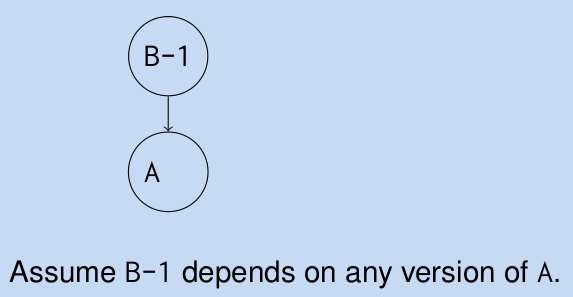
\includegraphics[height=5cm]{image201110/cabal-1.png}
  \end{center}
  \label{fig:cabal-1}\caption{Hackage DB上でB-1パッケージがAに依存している場合}
\end{figure}

まず上図のようにHackage DBでB-1パッケージがAパッケージに依存している場合を
考えます。この時B-1はAのバージョンについて特に指定していないとします。

\begin{figure}[ht]
  \begin{center}
    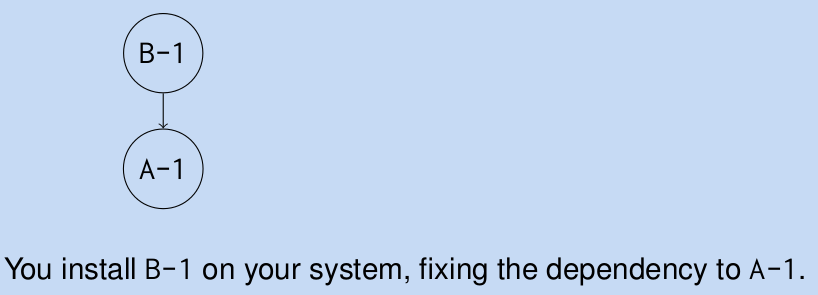
\includegraphics[height=5cm]{image201110/cabal-2.png}
  \end{center}
  \label{fig:cabal-2}\caption{B-1とA-1をインストール}
\end{figure}

このようなHackage DBからB-1をインストールするとAパッケージの最新バージョン
であるA-1も一緒にインストールされます。

\begin{figure}[ht]
  \begin{center}
    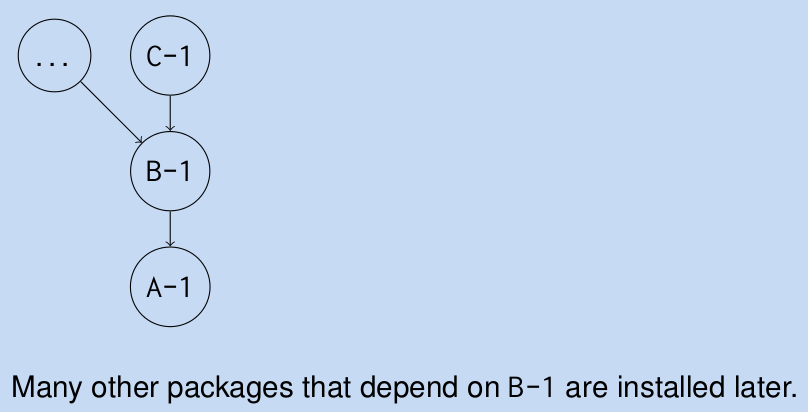
\includegraphics[height=5cm]{image201110/cabal-3.png}
  \end{center}
  \label{fig:cabal-3}\caption{そしてさらにB-1に依存したHackage群をインストール}
\end{figure}

そうして、このような環境にさらにC-1を含むB-1依存したHackage群をインストール
します。ここで、Bに依存しているC-1はローカルではB-1に紐づけられています。

\begin{figure}[ht]
  \begin{center}
    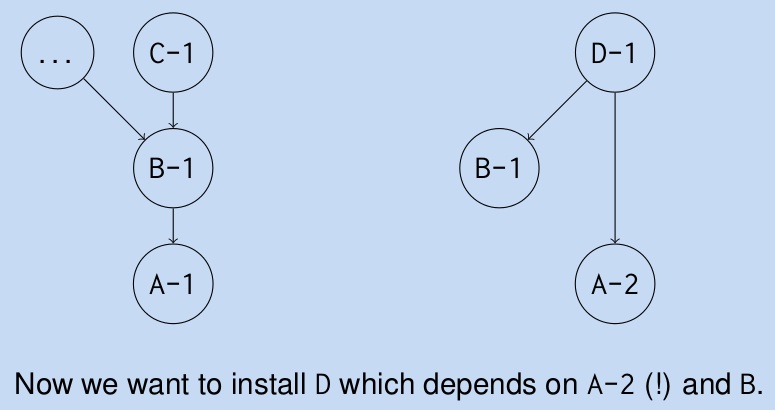
\includegraphics[height=5cm]{image201110/cabal-4.png}
  \end{center}
  \label{fig:cabal-4}\caption{A-2に依存しているD-1をインストールしようと試みる}
\end{figure}

ここでHackage DBからD-1をインストールしてみましょう。
D-1はHackage DB上(上図右)ではA-2とB-1にバージョン指定で依存しています。
ローカルにはA-1とB-1がインストールされています。

\begin{figure}[ht]
  \begin{center}
    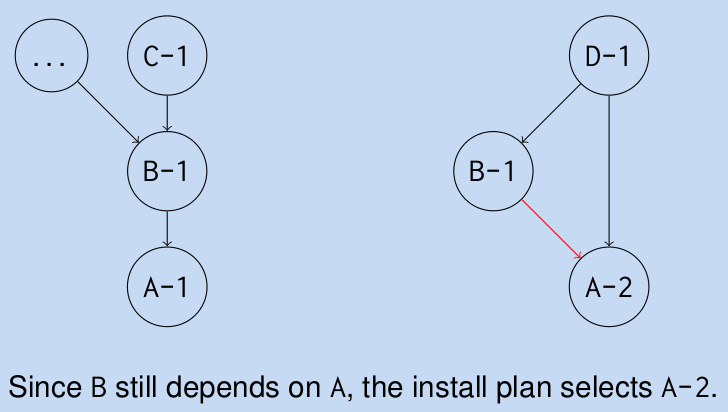
\includegraphics[height=5cm]{image201110/cabal-5.png}
  \end{center}
  \label{fig:cabal-5}\caption{cabalはD-1をインストールにあたってA-2もインストールしようとする}
\end{figure}

このままローカルにインストールされているA-1とB-1を無変更でD-1をインストール
することはできません。そこで、cabalはインストール計画をたて、
A-1のかわりにA-2をインストールしようとします。

\begin{figure}[ht]
  \begin{center}
    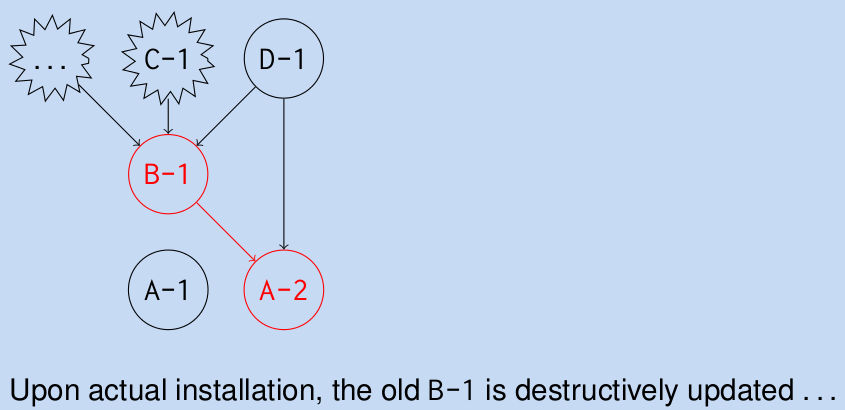
\includegraphics[height=5cm]{image201110/cabal-6.png}
  \end{center}
  \label{fig:cabal-6}\caption{D-1は正常にインストールされたが、B-1に依存していたHackage群は依存が壊れてしまう}
\end{figure}

A-2,B-1,D-1について\texttt{cabal}はインストール/更新を完了しました。
しかし、B-1に依存していたHackageについては再コンパイルは行ないません。
当然B-1に依存していたHackageは依存が壊れたまま放置されてしまうことになります。


この問題は依存解決する際のインストール計画の際にバックトラックが行なわれない
ためです。B-1を再インストールするのであれば、それに依存したHackage(C-1など)
も再インストールすべきだったのです。
もちろんHaskellコミュニティではこの問題を認識しており、その解決のために
新しいソルバを実装しています。
\footnote{\url{http://darcs.haskell.org/cabal-branches/cabal-modular-solver}}
近い将来に本家\texttt{cabal}に取り込まれることでしょう。

\subsubsection{Hackageが依存する環境についてcabalコマンドは面倒をみてくれない}

cairo
\footnote{\url{http://hackage.haskell.org/package/cairo}}
のようにC言語に依存するHackageについてはcabalコマンドは面倒を見てくれません。
Debianパッケージlibcairo2-devが入っていない環境で
cairo Hackageを\texttt{cabal}コマンドを使ってインストールしようとしても、
(当然)コンパイルエラーによってインストールに失敗します。

そもそもDebianではHaskell以外の部分のパッケージはDebianパッケージ(deb)によって管理されています。
cabalコマンドはOSに依存していないので、(当然)apt-getを呼び出すわけにもいきません。
\footnote{\url{http://packages.debian.org/ja/sid/auto-apt}
を使ってcabalコマンド実行の裏でDebianパッケージを自動インストールする手はあるかもしれませんね ;-)}

\subsubsection{Hackage群全てを最新バージョンでインストールできないかもしれない}

yesod \footnote{\url{http://hackage.haskell.org/package/yesod}}
,hakyll \footnote{\url{http://hackage.haskell.org/package/hakyll}}
,hamlet \footnote{\url{http://hackage.haskell.org/package/hamlet}}
の3つのHackageを例に説明します。
この問題はyesod-0.9.2, hakyll-3.2.0.8, hamlet-0.10.2のバージョン間で生じていました。(現在は解消されています)

まずそれぞれのHackageについて依存を見てみましょう。

\begin{commandline}
$ cabal info yesod-0.9.2
* yesod-0.9.2            (program and library)
--snip--
    Dependencies:  yesod-core >=0.9.1.1 && <0.10, yesod-auth ==0.7.*,
--snip--
                   hamlet ==0.10.*, shakespeare-js ==0.10.*,
--snip--
$ cabal info hakyll-3.2.0.8
* hakyll-3.2.0.8           (library)
--snip--
    Dependencies:  base ==4.*, binary >=0.5 && <1.0, blaze-html >=0.4 && <0.6,
--snip--
                   filepath >=1.0 && <2.0, hamlet >=0.7 && <0.9,
\end{commandline}

あれ?yesod-0.9.2はhamlet-0.10.*に依存しているのにhakyll-3.2.0.8は
hamlet-0.7.*もしくはhamlet-0.8.*に依存しています。
確かに表面上問題はありません。この状態でもyesodとhakyllの両方をインストール
することはできます。しかしもしhakyllとyesod両方のライブラリを使いたいプログラム
を作りたくなった場合にはどうしたら良いのでしょう?
hakyllはローカルでWebサーバを起動してプレビューする機能を持っています。
たまたまhakyllはこのWebサーバのエンジンとしてsnap
\footnote{\url{http://hackage.haskell.org/package/snap}}
を使っていたから良かったもののyesodを使っていたら、古いyesodの機能
しか使えないところです。

どうしてこんな状態でHackageが放置されていたのでしょう?
やる気がないのでしょうか?いえいえそんなことはありません。
今度はhamletについて調べてみましょう。

\begin{multicols}{2}
hamlet-0.8.2.1のModuleリスト
\begin{commandline}
Text
  Text.Cassius
  Text.Coffee
  Text.Hamlet
    Text.Hamlet.NonPoly
    Text.Hamlet.RT
  Text.Julius
  Text.Lucius
  Text.Romeo
  Text.Shakespeare
\end{commandline}
\columnbreak
hamlet-0.9.0のModuleリスト
\begin{commandline}
Text
  Text.Cassius
  Text.Coffee
  Text.Hamlet
  Text.Julius
  Text.Lucius
  Text.Romeo
  Text.Shakespeare
\end{commandline}
\end{multicols}

あれ?APIに変更があるようです。ここで注目したいのはText.Hamlet.RTモジュールが
消滅していることです。
嫌な予感がします。hakyllのソースコード
\footnote{\url{https://github.com/jaspervdj/hakyll/blob/master/src/Hakyll/Web/Template/Read/Hamlet.hs}}
を見てみましょう。

\begin{commandline}
-- | Read templates in the hamlet format
--
{-# LANGUAGE MultiParamTypeClasses #-}
module Hakyll.Web.Template.Read.Hamlet
    ( readHamletTemplate
    , readHamletTemplateWith
    ) where

import Text.Hamlet (HamletSettings, defaultHamletSettings)
import Text.Hamlet.RT

import Hakyll.Web.Template.Internal
--snip--
\end{commandline}

あーhakyllのコンパイルにはText.Hamlet.RTモジュールが必須なんですね。
これでは新しいhamletを使うことができない訳です。

Hackage作者が自由に依存Hackageのバージョンを選択可能である以上、
このようなHackage群全体の不整合は避けられません。

\subsection{HackageをDebianパッケージ化する}

cabalを使ってDebianパッケージと同等のレベルで
パッケージ管理をするのは現状では難しいことがわかりました。
それにapt-getでライブラリ環境が整うのはDebianユーザとしてうれしいですよね。
そこで、自分の良く使うHackageはDebianパッケージ化してDebian本体に
登録してしまうのはいかがでしょうか。
実はHackageをDebianパッケージ化するのはすごく簡単です。
\texttt{cabal-debian}というまんまの名前のコマンドがあります。\footnote{\url{http://hackage.haskell.org/package/debian}}
さっそくやってみましょう!

例題としてHCWiid
\footnote{Wiiリモコンからイベントを拾うためのライブラリ
  \url{http://hackage.haskell.org/package/hcwiid}}
をDebianパッケージ化してみます。
まずHackageのDebianパッケージ化に必要なhaskell-debian-utils,
haskell-devscriptsをapt-get installしましょう。

\begin{commandline}
$ sudo apt-get install haskell-debian-utils haskell-devscripts
$ rehash
\end{commandline}

hackageをダウンロードして解凍したら、ディレクトリに移動しておもむろに\texttt{cabal-debian}コマンドを使います。

\begin{commandline}
$ wget http://hackage.haskell.org/packages/archive/hcwiid/0.0.1/hcwiid-0.0.1.tar.gz
$ tar xfz hcwiid-0.0.1.tar.gz
$ cd hcwiid-0.0.1/
$ cabal-debian --debianize --ghc --maintainer="Kiwamu Okabe <kiwamu@debian.or.jp>"
$ ls debian
changelog  compat  control  copyright  rules*
$ debuild -rfakeroot -us -uc
--snip--
 dpkg-genchanges  >../haskell-hcwiid_0.0.1-1~hackage1_amd64.changes
dpkg-genchanges: including full source code in upload
 dpkg-source --after-build hcwiid-0.0.1
dpkg-buildpackage: full upload; Debian-native package (full source is included)
Now running lintian...
W: haskell-hcwiid source: native-package-with-dash-version
W: haskell-hcwiid source: out-of-date-standards-version 3.9.1 (current is 3.9.2)
E: libghc-hcwiid-dev: copyright-file-contains-full-gpl-license
E: libghc-hcwiid-dev: copyright-should-refer-to-common-license-file-for-lgpl
E: libghc-hcwiid-dev: description-contains-tabs
E: libghc-hcwiid-prof: copyright-file-contains-full-gpl-license
E: libghc-hcwiid-prof: copyright-should-refer-to-common-license-file-for-lgpl
E: libghc-hcwiid-prof: description-contains-tabs
E: libghc-hcwiid-doc: copyright-file-contains-full-gpl-license
E: libghc-hcwiid-doc: copyright-should-refer-to-common-license-file-for-lgpl
E: libghc-hcwiid-doc: description-contains-tabs
Finished running lintian.
$ ls ../*hcwiid*deb
../libghc-hcwiid-dev_0.0.1-1~hackage1_amd64.deb
../libghc-hcwiid-doc_0.0.1-1~hackage1_all.deb
../libghc-hcwiid-prof_0.0.1-1~hackage1_amd64.deb
\end{commandline}

なんかあっさりDebianパッケージができちゃいました。
lintianがなんか言ってますが、
あまり深刻なものではないのでとりあえずインストールしてみましょう。

\begin{commandline}
$ sudo dpkg -i ../libghc-hcwiid-dev_0.0.1-1\~hackage1_amd64.deb \
../libghc-hcwiid-doc_0.0.1-1\~hackage1_all.deb ../libghc-hcwiid-prof_0.0.1-1\~hackage1_amd64.deb
$ cd ~/
$ rm -rf .ghc .cabal # これでcabalでインストールしたパッケージは一切使っていないはずです
$ ghc-pkg list|grep hcwiid
    hcwiid-0.0.1
\end{commandline}
Hackageはインストール済みのようです。hcwiidライブラリを使ってみましょう。

Test.hs
\begin{commandline}
module Main where

import Prelude
import Control.Monad
import System.CWiid
import System.Posix.Unistd

main :: IO ()
main = do
  putStrLn "Put Wiimote in discoverable mode now (press 1+2)..."
  (Just wm) <- cwiidOpen
  putStrLn "found!"
  _ <- cwiidSetLed wm
  _ <- cwiidSetRptMode wm
  _ <- forever $ do _ <- usleep 300000
                    cwiidGetBtnState wm >>= print
  return () -- not reach
$ ghc --make Test.hs
[1 of 1] Compiling Main             ( Test.hs, Test.o )
Linking Test ...
$ ./Test
Put Wiimote in discoverable mode now (press 1+2)...
\end{commandline}

なんて簡単なんでしょう!簡単なHackageならcabal-debianコマンドを使えば
Debianパッケージ化が完了してしまうようです。
しかも下記3つのライブラリに分割してくれています。やった!

\begin{itemize}
 \item libghc-HOGE-dev  - 通常使用するライブラリ
 \item libghc-HOGE-doc  - Haddockで生成されたAPIドキュメント
 \item libghc-HOGE-prof - プロファイラ対応ライブラリ
\end{itemize}

\subsection{haskell-debian-utilsのしくみ}

cabal-debianでのDebianパッケージ化はどのようなしくみなのでしょうか。
さきほど作ったhcwiidパッケージのdebian/rulesファイルを見てみましょう。

\begin{commandline}
#!/usr/bin/make -f
include /usr/share/cdbs/1/rules/debhelper.mk
include /usr/share/cdbs/1/class/hlibrary.mk

# How to install an extra file into the documentation package
#binary-fixup/libghc-hcwiid-doc::
#       echo "Some informative text" > debian/libghc-hcwiid-doc/usr/share/doc/libghc-hcwiid-doc/AnExtraDocFile
\end{commandline}

なんということでしょう。内容がありません。。。
これはhlibrary.mkファイルに秘密があるに相違ありません。
全部を読まずにまずはlibghc-HOGE-devのbuildターゲットとその近辺をhlibrary.mk
から抜き出してみましょう。

\begin{commandline}
DEB_SETUP_BIN_NAME ?= debian/hlibrary.setup
BUILD_GHC := $(DEB_SETUP_BIN_NAME) build

$(DEB_SETUP_BIN_NAME):
        if test ! -e Setup.lhs -a ! -e Setup.hs; then echo "No setup script found!"; exit 1; fi
        for setup in Setup.lhs Setup.hs; do if test -e $$setup; then ghc --make $$setup -o $(DEB_SETUP_BIN_NAME); \
          exit 0; fi; done

build/libghc-$(CABAL_PACKAGE)-prof build/libghc-$(CABAL_PACKAGE)-dev:: build-ghc-stamp

build-ghc-stamp: dist-ghc
        $(BUILD_GHC) --builddir=dist-ghc
        touch build-ghc-stamp
\end{commandline}

なるほど。libghc-HOGE-devをbuildしようとすると、
まずSetup.lhsもしくはSetup.hsをghcを使ってコンパイルして\texttt{debian/hlibrary.setup}
コマンドを作成するようです。
そうして作ったdebian/hlibrary.setupコマンドを使って
"debian/hlibrary.setup build --builddir=dist-ghc"
のようにしてdist-ghcディレクトリ上でHackageをコンパイルするんですね。

ちょっと脱線しますが、
このビルドプロセスはcabalが普段やっていることと全く同じです。
cabalはインストール対象のHackageを取得/展開したら、まずこのSetup.hsを
ghcでコンパイルして、そのコンパイルした結果できた実行バイナリを
本当のビルダ/インストーラとして使います。
普段使っている/usr/bin/cabalコマンドは"cabal-install"と呼ばれています。
そして、Setup.hsを書くために必要なライブラリを"Cabal"と呼びます。
ややこしいですね。。。

ではlibghc-HOGE-devのinstallはどうなっているのでしょうか?

\begin{commandline}
debian/tmp-inst-ghc: $(DEB_SETUP_BIN_NAME) dist-ghc
	$(DEB_SETUP_BIN_NAME) copy --builddir=dist-ghc --destdir=debian/tmp-inst-ghc

install/libghc-$(CABAL_PACKAGE)-dev:: debian/tmp-inst-ghc debian/extra-depends
	cd debian/tmp-inst-ghc ; find usr/lib/haskell-packages/ghc/lib/ \
		\( ! -name "*_p.a" ! -name "*.p_hi" \) \
		-exec install -Dm 644 '{}' ../$(notdir $@)/'{}' ';'
	pkg_config=`$(DEB_SETUP_BIN_NAME) register --builddir=dist-ghc --gen-pkg-config | sed -r 's,.*: ,,'`; \
		$(if $(HASKELL_HIDE_PACKAGES),sed -i 's/^exposed: True$$/exposed: False/' $$pkg_config;) \
		install -Dm 644 $$pkg_config debian/$(notdir $@)/var/lib/ghc/package.conf.d/$$pkg_config; \
		rm -f $$pkg_config
	if [ 'z$(DEB_GHC_EXTRA_PACKAGES)' != 'z' ] ; then \
		echo '$(DEB_GHC_EXTRA_PACKAGES)' > \
                debian/$(notdir $@)/usr/lib/haskell-packages/ghc/lib/$(CABAL_PACKAGE)-$(CABAL_VERSION)/extra-packages ; \
	fi
	dh_haskell_provides -p$(notdir $@)
	dh_haskell_depends -p$(notdir $@)
	dh_haskell_shlibdeps -p$(notdir $@)
\end{commandline}

ちょっとわかりにくいですが、パッケージ化の後半はDebian流儀の詳細なので
踏みこまずに解釈すると、
まずlibghc-HOGE-devをinstallしようとすると、debian/tmp-inst-ghcターゲット
が呼び出されて
"debian/hlibrary.setup copy --builddir=dist-ghc --destdir=debian/tmp-inst-ghc"
のようなコマンドが実行されて、dist-ghcでコンパイルした内容が
debian/tmp-inst-ghc以下にインストールされます。
あとは、Debianの流儀にのっとってdebian/tmp-inst-ghc以下のファイル群を
パッケージ化するだけです。
パッケージ化対象のHackageが依存しているHackageも
dh\_haskell\_shlibdepsでちゃんと検出してくれるみたいです。 :)

\subsection{作ったパッケージをDebianに登録するには}

せっかく作ったHackageです。自分だけで使っているのはもったいないです。
Debian本家に登録して皆に使ってもらいましょう!
Debian本家に登録しておけばめぐりめぐってUbuntuにも登録されるかもしれませんよ?

その秘技はプレゼン資料の方でこっそり、あなただけに、紹介します。 ;)

%-------------------------------------------------------------------------------
\dancersection{月刊 debhelper 第1回}{岩松 信洋}
%-------------------------------------------------------------------------------
\index{げっかんでぶへるぱー@月刊Debhelper}
\index{debhelper}

\subsection{debhelper とは何か?}

Debian パッケージを作成する時、パッケージに必要なファイルのチェック、
コンパイル前の設定、コンパイルなど様々な処理を行う必要があります。
Debianパッケージでは debian/rules という GNU Make のmakefile に各処理
を記述するのですが、細かい処理をひとつづつ書いていくと膨大な量になります。

またコードの量が多くなるとバグも多くなり、パッケージ作成時に問題が起きた
ときに修正するのは大変です。
これらの処理を機能毎にまとめ、使いやすくした機能を提供しているパッケージ
として debhelper があります。他にも同様のツールがいくつかありますが、
1番使われているのがこの debhelper です。
Debian パッケージをメンテナンスしている人にとって debhelper の知識が必須と
言ってもいいでしょう。

ちなみにdebhelper は Debian 開発者の Joey Hess 氏\footnote{Wikiエンジンのikiwiki, 
ディストリビューションのパッケージ間変換ツールである alien の開発者として有名。}
によって開発/メンテナンスされ、最新のバージョンは 8.9.8 となっています。

\subsection{月刊 debhelperとは?}
先にも説明したように、Debian パッケージをメンテナンスしている人にとって 
debhelper の知識が必須となっています。
debhelper がどのような機能を提供して、それらをどのように使えばいいのか、
どのように使われているのか、理解しておく必要があります。
現時点で debhelper では59個のコマンド(dh\_で始まるコマンド)が提供されており、
全部理解するのは難しいでしょう。また、debhelper に収録されていない debhelper サポートツール
を含めると100個ほどになります。
日頃Debianの開発を行なっている人でも「ああ、こんな機能があるのだ」と思うことがあるぐらいです。
更にdebhelper 7 からコマンドがいくつか増え、debian/rules ファイルが以下のように記述
できるようになりました。

これだけでは何をやっているのかさっぱり分かりません。
細かい指定を行いたい場合、どのようにしたらいいのかすらわからない状態です。

そこで debhelper で提供されているコマンドの動きと使い方を毎月数個づつ
紹介し、Debian勉強会参加者でパッケージ作成の理解を深める企画、「月刊 debhelper」
を企画しました。
全て理解した頃には、皆 Debian パッケージメンテナになっているかもしれません。
ヒャッハー!

\begin{multicols}{2}

\begin{commandline}
debhelper 6:
#!/usr/bin/make -f

build: build-stamp
build-stamp:
    dh_testdir
    $(MAKE)
    touch $@

clean:
    dh_testdir
    dh_testroot
    $(MAKE) clean
    dh_clean

install: build
    dh_testdir
    dh_testroot
    dh_clean -k

binary-indep:

binary-arch: build install
    dh_testdir
    dh_testroot
    dh_installchangelogs ChangeLog
    dh_installd
.....
\end{commandline}
\columnbreak
\begin{commandline}
debhelper 7:
#!/usr/bin/make -f
%:
        dh $@
\end{commandline}
\end{multicols}
% $

\subsection{debian パッケージ構築、全体の流れ}

いきなり個々のコマンド説明をしてもよくわからないので、パッケージ作成の全体の
流れとどのようなコマンドが呼び出されるのか説明します。
Debian パッケージが作成される簡単流れは以下の通りで、
図にすると図\ref{fig:rules-work}のようになります。

\begin{enumerate}
\item パッケージビルド環境を構築する

実際にビルドを始める前に、まずはビルドのための環境を構築する必要があります。
ここでは、ソースコードの展開、パッケージ構築依存のチェック等を行います。

\item 不要なファイルを削除する\\
次にパッケージに不要なファイルを削除します。 
例えば、前に行われたパッケージビルドで生成されたファイルがある場合はそれを削除して、 
ソースが展開された常に同じ状態からビルドできるようにします。 

これは debian/rules ファイルの {\bf clean} ターゲットで行われ、このターゲットは
「不要なファイルを削除する」ことを目的とするように Debian Policy で定められています。

また clean ターゲットでは、以下の dehhelper コマンドが実行されます。
\begin{commandline}
dh_testdir -> dh_auto_clean -> dh_clean
\end{commandline}

\item  バイナリパッケージに格納するファイルをビルドする

次にソースコードからバイナリをビルドします。ここではconfigure などを使った
コンパイル前の設定、コンパイラを使った実行ファイルの作成、ドキュメントの変
換などがおこなわれます。

これは debian/rules ファイルの {\bf build} ターゲットで行われ、このターゲットは
「プログラムの設定、コンパイルやデータの変換」ことを目的とするように Debian Policy で
定められています。

また build ターゲットでは、以下の dehhelper コマンドが実行されます。
\begin{commandline}
dh_testdir -> dh_auto_configure -> dh_auto_build -> dh_auto_test
\end{commandline}

\item ビルドしたファイルをバイナリパッケージにまとめる

必要なファイルをすべてビルド完了した後、それらを適切なパーミッションで
適切な場所に配置し、バイナリパッケージにまとめます。 

ここでは、debian/tmpを/(ルート)と見なしてソフトウェア全体の
インストール (「仮インストール」) を行い、 その上でdebian/tmp 内の各ファイルを適切に
debian/バイナリパッケージ名に振り分け、 最後にdebian/バイナリパッケージ名をそれぞれ
バイナリパッケージ化する、という流れで行います。 debian/バイナリパッケージ名 を
バイナリパッケージ化する際には、各ファイルのパーミッションの設定やファイルの圧縮など、
行わなければならないことや、推奨されていることが多数あります。 

これは debian/rules ファイルの {\bf binary、binary-arch、 binary-indep} 
ターゲットで行われ、このターゲットは
「バイナリパッケージとしてまとめる」ことを目的とするように Debian Policy で
定められています。

また binary、binary-arch、 binary-indep ターゲットでは、以下の dehhelper コマンドが実行されます。
\begin{commandline}
dh_testdir -> dh_auto_configure -> dh_auto_build -> dh_auto_test -> dh_testroot
-> dh_prep -> dh_installdirs -> dh_auto_install -> dh_install -> dh_installdocs
-> dh_installchangelogs -> dh_installexamples -> dh_installman -> dh_installcatalogs
-> dh_installcron -> dh_installdebconf -> dh_installemacsen -> dh_installifupdown
-> dh_installinfo -> dh_pysupport -> dh_installinit -> dh_installmenu -> dh_installmime
-> dh_installmodules -> dh_installlogcheck -> dh_installlogrotate -> dh_installpam
-> dh_installppp -> dh_installudev -> dh_installwm -> dh_installxfonts -> dh_installgsettings
-> dh_bugfiles -> dh_ucf -> dh_lintian -> dh_gconf -> dh_icons -> dh_perl -> dh_usrlocal
-> dh_link -> dh_compress -> dh_fixperms -> dh_strip -> dh_makeshlibs -> dh_shlibdeps
-> dh_installdeb -> dh_gencontrol -> dh_md5sums -> dh_builddeb
\end{commandline}

\item .changesファイルを作成する

パッケージが作成されたら、そのパッケージの.changelog ファイルを作成します。
このファイルの作成には dpkg-genchanges コマンドが使われます。
このコマンドは debhelper のコマンドではありません。
\item パッケージに署名する

必須ではありませんが、パッケージができたら.dscファイルと.changes ファイルに
GPG/PGPを使って署名をします。この署名には debsign コマンドを使います。
このコマンドは debhelper のコマンドではありません。
\end{enumerate}

\begin{figure}[ht]
  \begin{center}
    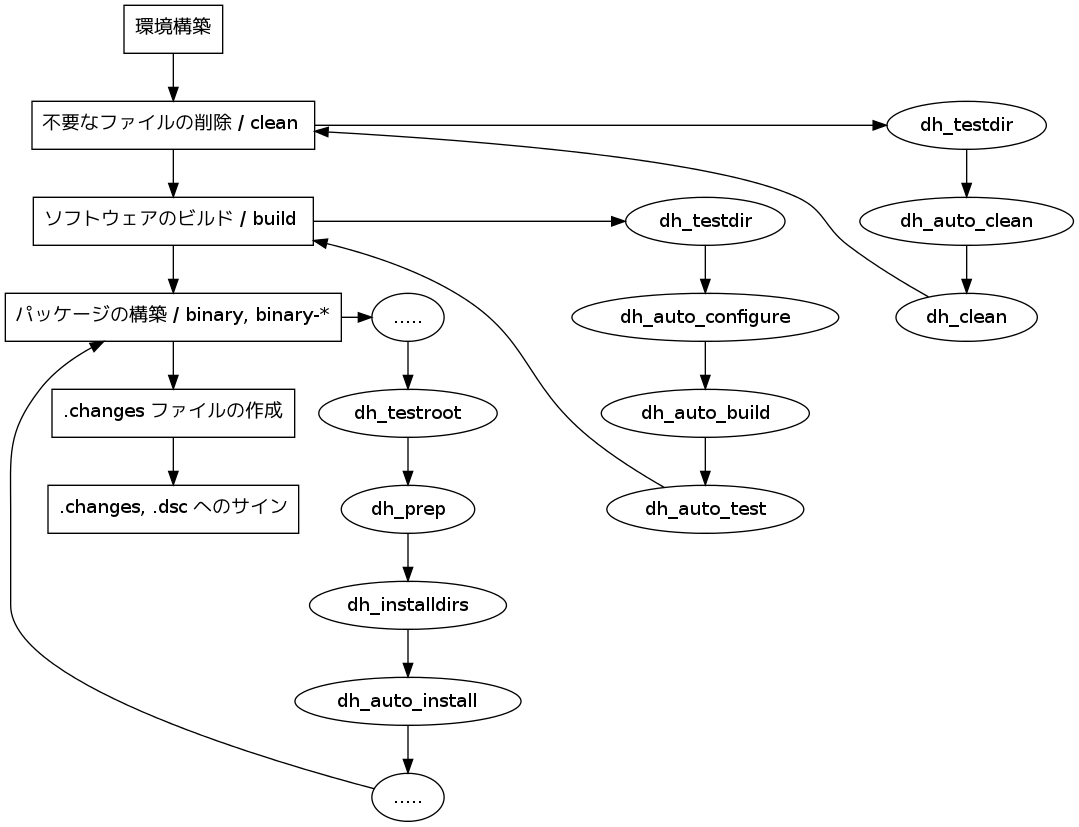
\includegraphics[height=10cm]{image201110/rules-work.png}
  \end{center}
  \label{fig:rules-work}\caption{各処理とdebhelperコマンドの関係図}
\end{figure}

\subsection{その他 debhelper の重要な機能}

\subsubsection{環境にあわせたシーケンス情報を読み込む}
debhelper は特定の言語や環境に合わせたシーケンスを定義し、
読み込ませることによって、makefile 内で利用できるターゲットとコマンドを増やすことができます。
例えば、パッチ管理ツールである quilt を使ったターゲットは debhelper には含まれていません。
使いたい場合には、{\bf --with}オプションを使って指定します。

\begin{commandline}
%:
        dh $@ --with quilt
\end{commandline}
指定することによって、\bf{dh\_quilt\_patch}が利用できるようになります。

\subsubsection{各 debhelper コマンドの動きを変更する}
上記で説明しように、debhelper では各ターゲットと各コマンドの動作が予め決められています。
これらを変更するには各コマンド用のターゲットに対して動作を記述します。
このターゲットは {\bf override\_各debhelper コマンド}となっており、dh\_auto\_configure
(決められた値で自動的に configure を実行するためのコマンド)の場合には以下のように使います。

\begin{commandline}
override_dh_auto_configure:
    dh_auto_configure -- --enable-foo
\end{commandline}

\subsection{今月のコマンド : dh\_testdir}

\subsubsection{概要}

パッケージビルドを行うときに正しいディレクトリにいるかチェックします。

\subsubsection{使い方}

dh\_testdir コマンドはカレントディレクトリに debian/control があることに
よって正しいディレクトリにいるかチェックをしています。
dh\_testdir はほとんどのターゲットから利用されます。ちゃんと debian パッケージ
をビルドできる場所にいるかチェックするためです。


\begin{commandline}
$ mkdir foo
$ cd foo
$ dh_testdir
dh_testdir: cannot read debian/control: そのようなファイルやディレクトリはありません
echo $?
2
$ mkdir debian
$ touch debian/control
$ dh_testdir
$ echo $?
0
\end{commandline}
%$

引数としてファイルパスを指定することができます。
ファイルパスを指定した場合には、指定したファイルによってチェックが行われます。

\begin{commandline}
$ touch moo
$ dh_testdir moo
$ echo $?
0
\end{commandline}
%$

\subsection{今月のコマンド : dh\_bugfiles}

\subsubsection{概要}

dh\_bugfiles コマンドは バグレポートに必要なファイルをパッケージに
格納します。
バグレポートに使うファイルは script、control、presubj の3つがあり、
debian/bug ディレクトリに格納されている必要があります。
各ファイルの用途を以下に説明します。

\begin{itemize}
\item script

バグレポート用のスクリプトです。
バグレポートを行うためのツールreportbugs 等でレポート作成時に呼び出し、
結果をバグレポートの一部として追記します。
例えば、X.Orgのドライバ群は /usr/share/bug/xserver-xorg-core/script 
にシンボリックリングを張ったファイルをバイナリパッケージ内に持ちます。
このスクリプトでは、reportbug を実行した環境のカーネルバージョンや 
dmesg, xorg のログなどが自動的に出力されるようになっています。

\item control

controlファイルは指定したコマンドの結果をバグレポートの一部として出力します。
コマンドには以下の4つがあります。

\begin{itemize}
\item package-status
指定したパッケージのステータス(インストール状態、バージョン)を
バグレポートに追加します。

\begin{commandline}
設定例:
/usr/share/bug/mutt/control package-status: mutt mutt-patched mutt-dbg
\end{commandline}

\item report-with
指定したパッケージ情報をバグレポートに追加します。

\begin{commandline}
設定例:
/usr/share/bug/xorg/control report-with: xserver-xorg
\end{commandline}

\item Send-To
Debian BTS以外に自動的にが行われるメールアドレスを設定します。

\begin{commandline}
Send-To: foo@example.org
\end{commandline}

\item Submit-As:
一つのパッケージにレポートが行われるようにコントールする
以下のように設定した場合、linux-image-3.0.0-2-amd64 にバグレポート
した場合には linux-2.6 に行われるように自動的に変更されます。

\begin{commandline}
control:Submit-As: linux-2.6
\end{commandline}
\end{itemize}

\item presubj

レポートする前の警告文を出すために使います。
例えば、gnupg パッケージの場合にはこのファイルに
\begin{commandline}
Please consider reading /usr/share/doc/gnupg/README.BUGS.Debian before
sending a bug report. Maybe you'll find your problem there.
\end{commandline}
と書くことによって、バグレポートを送る前に /usr/share/doc/gnupg/README.BUGS.Debian 
を参照するよう、誘導しています。

reportbug を使って、gnupg パッケージにバグレポートしようとしたとき、以下のような
メッセージが表示されます。
\begin{commandline}
Please consider reading /usr/share/doc/gnupg/README.BUGS.Debian before
sending a bug report. Maybe you'll find your problem there.


(You may need to press 'q' to exit your pager and continue using
reportbug at this point.)
\end{commandline}

\end{itemize}

これらのファイルは一つだけでもかまいません。

\subsubsection{使い方}

このコマンドは install ターゲットで使用します。

\begin{commandline}
install:
    ....
    dh_bugfiles
    ....
\end{commandline}

\subsection{次の発表者}
次の発表者は 勉強会で発表します。選ばれた人、おめでとうございます。
頑張ってください。

\printindex

\cleartooddpage

\vspace*{15cm}
\hrule
\vspace{2mm}

\includegraphics[width=2cm]{image200502/openlogo-nd.eps}
\noindent \Large \bf Debian 勉強会資料\\
\noindent \normalfont \debmtgyear{}年\debmtgmonth{}月\debmtgdate{}日 \hspace{5mm}  初版第1刷発行\\
\noindent \normalfont 東京エリア Debian 勉強会 (編集・印刷・発行)\\
\hrule

\end{document}
